\documentclass[10pt,a4paper,twocolumn]{article}

\usepackage[a4paper,margin=2cm,columnsep=0.7cm]{geometry}

\usepackage{fontspec}
\setmainfont{texgyretermes}[Path=fonts/, Extension=.otf, UprightFont=*-regular, BoldFont=*-bold, ItalicFont=*-italic, BoldItalicFont=*-bolditalic]
\usepackage{amsmath}
\usepackage{booktabs}
\usepackage[table]{xcolor}
\usepackage{tikz}
\usepackage{titlesec}
\usepackage{ragged2e}
\usepackage{url}

\definecolor{accent}{HTML}{000000}

\titleformat{\section}
  {\color{accent}\bfseries\large}{\thesection.}{0.5em}{}
\titleformat{\subsection}
  {\color{accent}\bfseries\normalsize}{\thesubsection}{0.5em}{}
\titlespacing*{\section}{0pt}{1.4ex plus .2ex}{0.3ex}

\setlength{\parindent}{0pt}
\setlength{\parskip}{0.5em}

\title{\vspace{-1.5em}\bfseries\color{accent}\Large Fondasi Sistem Keuangan Pribadi: Tiga Pilar}
\author{}
\date{}

\begin{document}

\twocolumn[
  \begin{@twocolumnfalse}
    \maketitle
    \vspace{-3.8em}
    \begin{center}
      \small Nonthawit Doungsodsri\\
      nonthawit.com\\
      3 Juni 2026\\
      Versi 1.0.0
    \end{center}
    \vspace{0.5em}
    \begin{quote}
      \normalsize\textbf{Abstrak} --- Makalah ini memaparkan kerangka kerja yang sederhana namun tahan lama untuk membangun keuangan pribadi, yakni ``Sistem Tiga Pilar'': Manajemen Arus Kas (Cashflow), Investasi, dan Menabung (pelestarian nilai). Argumen utamanya adalah bahwa keberhasilan finansial jangka panjang tidak berasal dari strategi yang canggih, melainkan dari \textbf{disiplin} dan kekonsistenan dalam menjalankan sistem yang dimiliki sendiri selama lima hingga sepuluh tahun atau lebih.
    \end{quote}
    \vspace{1em}
  \end{@twocolumnfalse}
]

\section{Pendahuluan}
Keuangan pribadi adalah pengelolaan uang milik sendiri yang selaras dengan tujuan hidup. Bagi kebanyakan orang, masalahnya bukan terletak pada penghasilan yang terlalu kecil, melainkan pada tidak adanya \textit{sistem} yang jelas untuk mengelola uang yang sudah diperoleh. Makalah ini menawarkan sistem nyata yang dapat digunakan seumur hidup, berpijak pada satu persamaan fondasi.

\begin{center}
{\setlength{\fboxsep}{10pt}\fbox{$\displaystyle \text{Pemasukan} \;-\; \text{Pengeluaran} \;=\; \text{Dana Kebebasan}$}}
\end{center}

``Dana Kebebasan'' adalah bahan baku kebebasan finansial. Jika hasilnya negatif, tujuan pertama adalah menjadikannya positif. Jika sudah positif, pertanyaan berikutnya adalah bagaimana cara mengalokasikannya. Jawaban makalah ini adalah menyalurkan Dana Kebebasan ke dalam tiga pilar yang bekerja bersama: Manajemen Arus Kas, Investasi, dan Menabung. Setiap pilar memiliki peran dan tujuannya masing-masing, sebagaimana dijelaskan secara berurutan di bawah ini.

\section{Pilar 1 --- Manajemen Arus Kas (Cashflow)}
\textbf{Apa itu.} Manajemen arus kas (Cashflow) berarti mengetahui berapa banyak uang yang masuk dan keluar setiap bulan, dengan mencatat pemasukan dan pengeluaran secara konsisten. Tidak diperlukan alat yang rumit; buku catatan sederhana atau aplikasi sudah lebih dari cukup. Kuncinya adalah kesinambungan, bukan kecanggihan.

\textbf{Tujuan.} Untuk mengetahui ``Dana Kebebasan'' yang sesungguhnya setiap bulan, yakni angka yang menunjukkan seberapa besar kapasitas Anda untuk berinvestasi dan menabung. Tanpanya, setiap rencana hanyalah perkiraan. Pilar ini adalah \textit{fondasi} tempat berdirinya pilar-pilar lain.

\textbf{Praktik.} Catat setiap hari atau setiap minggu hingga menjadi kebiasaan, tinjau total akhir bulan, pisahkan pengeluaran pokok dari pengeluaran bebas, dan usahakan agar ``Dana Kebebasan'' tetap positif sebelum melangkah ke pilar kedua dan ketiga.

\section{Pilar 2 --- Investasi}
\textbf{Apa itu.} Investasi berarti membuat uang Anda bekerja untuk Anda, menyalurkan Dana Kebebasan ke dalam imbal hasil jangka panjang. Berbeda dengan menyimpan uang tunai yang menganggur, uang yang diinvestasikan memiliki peluang untuk bertumbuh melalui bunga majemuk (compounding) seiring waktu.

\textbf{Tujuan.} Menghasilkan imbal hasil yang menumbuhkan kekayaan lebih cepat daripada sekadar menabung dan membawa Anda lebih dekat ke kebebasan finansial. Prinsip utamanya adalah \textbf{berinvestasi hanya pada hal yang benar-benar Anda pahami}. Berinvestasi karena ikut-ikutan, tanpa memahami aset yang bersangkutan, membuka pintu bagi risiko yang tidak terkendali.

\textbf{Praktik.} Jangan terburu-buru; berinvestasi ibarat menanam pohon, Anda tidak bisa memaksanya tumbuh. Mulailah dengan belajar hingga benar-benar paham, lalu gunakan \textbf{DCA} (Dollar-Cost Averaging): membeli aset secara rutin setiap bulan tanpa mempedulikan fluktuasi harga. Ini menghilangkan emosi dari pengambilan keputusan dan membangun disiplin investasi yang kokoh, sangat ideal bagi pemula. Namun demikian, DCA hanyalah salah satu dari sekian banyak cara untuk memulai investasi. Pendekatan lain juga tersedia, seperti investasi sekaligus (lump-sum), penyeimbangan ulang portofolio (rebalancing), atau value investing; masing-masing memiliki kekuatan tersendiri dan cocok untuk situasi yang berbeda. Pembaca sebaiknya mempelajari dan memilih metode yang sesuai dengan tujuan serta temperamen diri mereka.

\section{Pilar 3 --- Menabung (Pelestarian Nilai)}
\textbf{Apa itu.} Menabung di sini bukan berarti menumpuk uang tunai yang menganggur, melainkan memegang \textbf{aset yang memiliki daya preservasi nilai} guna mengurangi risiko dalam kehidupan. Uang tunai yang dibiarkan menganggur kehilangan daya beli setiap tahun akibat inflasi (inflation); menabung yang baik harus melindungi nilai uang Anda dari pengikisan tersebut.

\textbf{Tujuan.} Membangun rasa aman dan penyangga terhadap risiko, sehingga ketika hal yang tidak terduga terjadi, Anda memiliki aset yang mempertahankan nilainya sebagai sandaran. Pilar ini berperan sebagai ``pertahanan'' sementara pilar investasi berperan sebagai ``serangan''.

\textbf{Praktik.} Alih-alih terpaku pada satu jenis aset tertentu, pilihlah berdasarkan \textbf{kualitas} yang mumpuni dalam menjaga nilai, seperti ketahanan terhadap inflasi, likuiditas yang wajar, dan penerimaan yang luas. Contoh masa kini mencakup emas, reksa dana indeks (index fund), obligasi (bond), atau asuransi untuk mengalihkan risiko --- semuanya dapat berubah seiring perkembangan zaman. Oleh karena itu, pembaca sebaiknya mempelajari pilihan yang tersedia pada masa itu, mendiversifikasi agar risiko tidak terkonsentrasi pada satu aset, dan mempertahankan tingkat tabungan yang stabil sebagaimana dalam berinvestasi.

\section{Alokasi dan Disiplin}
Setelah memahami ketiga pilar, pertanyaan praktisnya adalah bagaimana membagi ``Dana Kebebasan'' di antara ketiganya. Ketiga pilar tersebut tidak berdiri sendiri; mereka bekerja bersama untuk menopang satu tujuan, kebebasan finansial, sebagaimana ditunjukkan pada Gambar~\ref{fig:pillars}.

\begin{figure}[t]
\centering
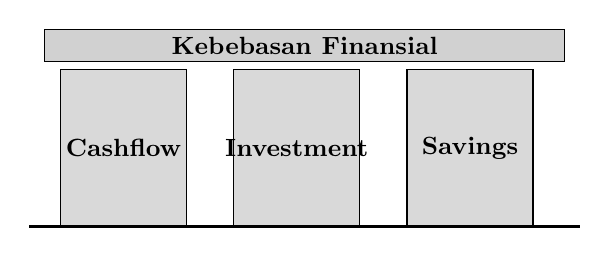
\begin{tikzpicture}[font=\small]
  \fill[accent!18] (-0.2,2.1) rectangle (6.4,2.5);
  \draw[accent] (-0.2,2.1) rectangle (6.4,2.5);
  \node[accent] at (3.1,2.3) {\bfseries Kebebasan Finansial};
  \foreach \x/\lbl in {0/Cashflow, 2.2/Investment, 4.4/Savings} {
    \fill[accent!15] (\x,0) rectangle (\x+1.6,2.0);
    \draw[accent] (\x,0) rectangle (\x+1.6,2.0);
    \node[accent,align=center] at (\x+0.8,1.0) {\bfseries \lbl};
  }
  \draw[accent,line width=1pt] (-0.4,0) -- (6.6,0);
\end{tikzpicture}
\caption{Tiga pilar yang menopang kebebasan finansial.}
\label{fig:pillars}
\end{figure}

\textbf{Contoh alokasi.} Misalkan pemasukan Rp~5{,}000{,}000 per bulan dengan pengeluaran pokok Rp~3{,}000{,}000, sehingga tersisa Rp~2{,}000{,}000 sebagai Dana Kebebasan. Dana Kebebasan ini dapat dibagi dengan rasio 30/40/30 sebagaimana pada Tabel~\ref{tab:alloc}. Yang perlu ditekankan adalah angka 30/40/30 hanyalah contoh ilustratif, bukan formula baku. Setiap orang memiliki penghasilan, kewajiban, tujuan, dan toleransi risiko yang berbeda; rasio yang cocok bagi satu orang belum tentu cocok bagi orang lain. Pembaca sebaiknya merancang rasio mereka sendiri berdasarkan kondisi nyata. Yang tidak boleh diabaikan adalah bahwa Dana Kebebasan harus selalu mengalir ke pilar \textbf{Investasi} dan \textbf{Menabung}; keduanya bersifat wajib dan setiap rencana harus menyertakannya. Seberapa besar proporsinya, dan bagaimana sisa Dana Kebebasan (seperti pengeluaran bebas atau tujuan lainnya) dialokasikan, pembaca bebas merancang sesuai kehidupan masing-masing.

\begin{table}[t]
\centering
\small
\begin{tabular}{lrr}
\toprule
\rowcolor{accent!15}
\textbf{Tujuan} & \textbf{Porsi} & \textbf{Jumlah (IDR)} \\
\midrule
Investasi          & 30\% & 600{,}000 \\
Menabung           & 40\% & 800{,}000 \\
Pengeluaran bebas  & 30\% & 600{,}000 \\
\midrule
\textbf{Total Dana Kebebasan} & \textbf{100\%} & \textbf{2{,}000{,}000} \\
\bottomrule
\end{tabular}
\caption{Contoh alokasi Dana Kebebasan Rp~2{,}000{,}000 (ilustratif).}
\label{tab:alloc}
\end{table}

\textbf{Disiplin adalah intinya.} Apapun cara Anda mengalokasikan, faktor penentu keberhasilan bukan terletak pada rasio maupun strategi yang rumit, melainkan pada \textbf{kekonsistenan dalam menjalankan sistem sendiri selama lima hingga sepuluh tahun atau lebih}. Kekuatan DCA dan menabung secara berkelanjutan baru akan terlihat nyata ketika Anda membiarkan waktu dan bunga majemuk (compounding) bekerja. Manfaat terdalam dari memiliki sebuah sistem adalah ia meredam pengaruh emosi --- baik keserakahan di pasar yang sedang naik maupun ketakutan di pasar yang bergejolak --- yang merupakan musuh sejati keuangan jangka panjang. Ketika Anda mengikuti sistem, keputusan bertumpu pada prinsip, bukan pada perasaan sesaat. Mereka yang memulai lebih awal dan tetap konsisten akan selalu mengungguli mereka yang cerdas tetapi berulang kali berhenti dan mulai lagi.

\section{Kesimpulan}
Membangun keuangan pribadi yang kokoh tidak memerlukan pengetahuan finansial tingkat tinggi ataupun strategi rahasia, hanya sebuah sistem yang mudah dipahami dan disiplin yang benar-benar dapat dijalankan. Ketiga pilar --- manajemen arus kas untuk mengetahui Dana Kebebasan, investasi untuk membuat uang bekerja bagi Anda, dan menabung untuk mengurangi risiko --- ketika dijalankan bersama secara konsisten, secara bertahap akan meningkatkan kualitas kehidupan finansial Anda sepanjang perjalanan.

Prinsip yang perlu selalu dibawa adalah: \textbf{``Mulailah dengan sistem yang sederhana, lalu jalankan secara konsisten.''} Waktu dan konsistensi adalah sekutu terkuat setiap investor.

\vspace{1em}
\noindent\rule{\linewidth}{0.4pt}\\
{\small\raggedright Dokumen ini adalah karya \textbf{Nonthawit Doungsodsri} --- dirilis untuk kepentingan publik. Pelajari lebih lanjut di nonthawit.com\par}

\end{document}
